\documentclass[10pt,a4paper]{article}
\usepackage[a4paper,margin=1.9cm,top=1.7cm,bottom=1.8cm]{geometry}
\usepackage[T1]{fontenc}
\usepackage[scaled=0.95]{helvet}
\renewcommand{\familydefault}{\sfdefault}
\usepackage{booktabs,tabularx,array,enumitem,listings,caption}
\usepackage{tikz}
\usetikzlibrary{positioning,arrows.meta,fit}
\usepackage{pgfplots}
\pgfplotsset{compat=1.18}
\usepackage{float,titlesec,needspace}
\titlespacing*{\section}{0pt}{12pt}{4pt}
\titlespacing*{\subsection}{0pt}{8pt}{2pt}
\usepackage[hidelinks]{hyperref}
\setlength{\parindent}{0pt}
\renewcommand{\topfraction}{0.9}\renewcommand{\bottomfraction}{0.8}\renewcommand{\textfraction}{0.07}\renewcommand{\floatpagefraction}{0.8}
\setlength{\textfloatsep}{8pt plus 2pt}\setlength{\intextsep}{8pt plus 2pt}
\setlength{\parskip}{5pt}
\setlist{nosep,leftmargin=1.5em,topsep=2pt}
\renewcommand{\arraystretch}{1.15}
\captionsetup{font=small,labelfont=bf,skip=4pt}
\lstset{basicstyle=\ttfamily\scriptsize,frame=single,framesep=4pt,breaklines=true,columns=fullflexible,
  keepspaces=true,showstringspaces=false,numbers=left,numberstyle=\tiny,numbersep=6pt,xleftmargin=14pt,
  captionpos=t,aboveskip=8pt,belowskip=4pt}
\renewcommand{\lstlistingname}{Code}
\newcolumntype{L}[1]{>{\raggedright\arraybackslash}p{#1}}
\tikzset{
  box/.style={draw,thick,rounded corners=2pt,align=center,font=\footnotesize,inner sep=4pt,minimum height=11mm},
  arr/.style={-{Stealth[length=2mm]},thick}}

\begin{document}

{\bfseries\LARGE Product Recommendation from Transaction History}\par
\vspace{2pt}
{\large Full project report: design, implementation and results}\par
\vspace{4pt}
Date: November 2026 \quad\textbar\quad Status: complete \quad\textbar\quad Model: Qwen3-1.7B (small language model), fine-tuned with LoRA
\vspace{6pt}
\hrule

\section*{Summary}
We built a system that reads a bank customer's recent transactions and profile, and predicts which of five products the customer is most likely to take up. The work covered four parts, all complete:
\begin{enumerate}
\item \textbf{Data.} A synthetic data generator, designed with a high-level and low-level design (HLD/LLD), produced 20,000 customers and 4.25 million transactions. Because the data is generated, the true chance of each customer taking each product is known.
\item \textbf{Model.} We fine-tuned an open small language model, Qwen3-1.7B, using LoRA. The model reads each customer's transactions as a sequence of compact codes, and it is trained together with a small network that reads the customer's profile.
\item \textbf{Training.} Two training rounds ran on Kaggle's free GPUs (two NVIDIA T4 cards, 16\,GB each). The second round took 6.4 hours in total.
\item \textbf{Evaluation.} The model was compared with four other models on 5,069 customers from later months than the training data.
\end{enumerate}
\textbf{Result.} Our model scored 0.736 AUC, 3.8\% below the standard LightGBM model (0.765). Transaction history on its own predicts take-up well above random (0.668), and the second round improved that figure from 0.623. To beat the standard model, the next step is to first teach the model general spending patterns on all transactions, and to train on more customers (Section~9).

%=====================================================================
\section{Problem and goals}
Banks usually summarise each customer into a set of totals, such as ``spend on groceries in the last 90 days'', and train a tree model such as LightGBM on those totals. Totals are quick to compute and work well, but they lose two kinds of information:
\begin{itemize}
\item \textbf{Order and timing.} A pay rise followed by transfers to a broker, and late fees followed by a quick loan, can add up to the same 90-day totals.
\item \textbf{Merchant detail.} Totals group shops into a few broad categories, so an airline and a bus company both become ``transport''.
\end{itemize}
\textbf{Goal.} Build a model that reads the transactions themselves, combines them with the profile, and recommends the best of five products: \emph{travel card, personal loan, investments, insurance} and \emph{cashback plus}. Measure it honestly against the standard approach.

\textbf{Constraints.} No real bank data was available, and training had to fit on free cloud GPUs (Kaggle, 2$\times$T4, 12-hour session limit).

%=====================================================================
\section{High-level design (HLD)}
\subsection{System overview}
The system has three stages: a data generator, a training pipeline and an evaluation stage. Figure~\ref{fig:hld} shows how they connect.

\begin{figure}[!htb]
\centering
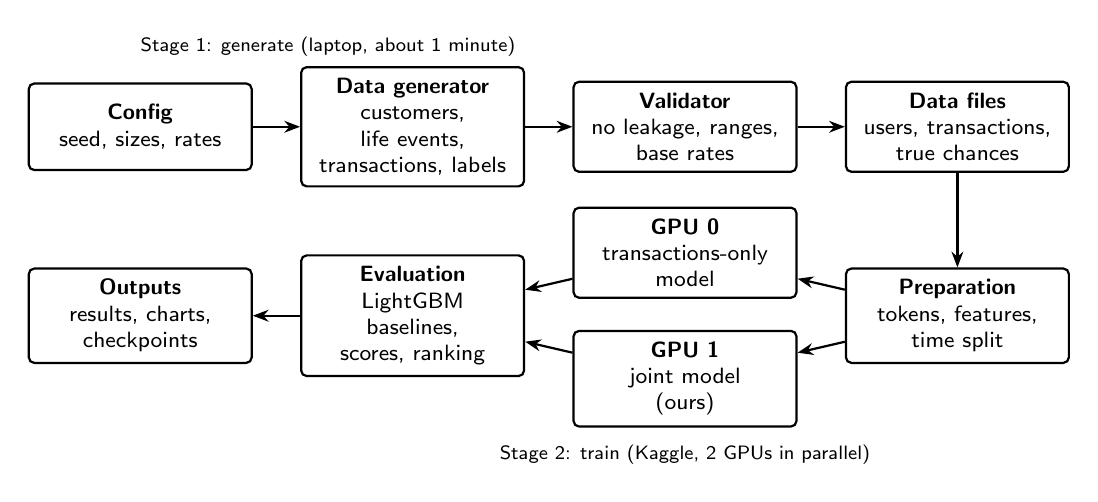
\begin{tikzpicture}[node distance=6mm and 6mm]
\node[box,text width=25.5mm] (cfg) {\textbf{Config}\\seed, sizes, rates};
\node[box,text width=25.5mm,right=of cfg] (gen) {\textbf{Data generator}\\customers, life events,\\transactions, labels};
\node[box,text width=25.5mm,right=of gen] (val) {\textbf{Validator}\\no leakage, ranges,\\base rates};
\node[box,text width=25.5mm,right=of val] (store) {\textbf{Data files}\\users, transactions,\\true chances};
\node[box,text width=25.5mm,below=12mm of store] (prep) {\textbf{Preparation}\\tokens, features,\\time split};
\node[box,text width=25.5mm,left=of prep,yshift=8mm] (g0) {\textbf{GPU 0}\\transactions-only\\model};
\node[box,text width=25.5mm,left=of prep,yshift=-8mm] (g1) {\textbf{GPU 1}\\joint model\\(ours)};
\node[box,text width=25.5mm,left=of g0,yshift=-8mm] (rep) {\textbf{Evaluation}\\LightGBM baselines,\\scores, ranking};
\node[box,text width=25.5mm,left=of rep] (out) {\textbf{Outputs}\\results, charts,\\checkpoints};
\draw[arr] (cfg) -- (gen); \draw[arr] (gen) -- (val); \draw[arr] (val) -- (store);
\draw[arr] (store) -- (prep); \draw[arr] (prep) -- (g0); \draw[arr] (prep) -- (g1);
\draw[arr] (g0) -- (rep); \draw[arr] (g1) -- (rep); \draw[arr] (rep) -- (out);
\node[font=\scriptsize,above=0mm of gen.north east,anchor=south east] {Stage 1: generate (laptop, about 1 minute)};
\node[font=\scriptsize,below=1mm of g1.south] {Stage 2: train (Kaggle, 2 GPUs in parallel)};
\end{tikzpicture}
\caption{High-level design. Stage 1 runs on a laptop; stages 2 and 3 run as one Kaggle job.}
\label{fig:hld}
\end{figure}

\subsection{Components}
\begin{tabularx}{\linewidth}{@{}L{3.2cm}X@{}}
\toprule
\textbf{Component} & \textbf{Responsibility} \\
\midrule
Data generator & Creates customers with hidden traits, plants life events, simulates 150 days of transactions, computes each customer's true chance of taking each product, chooses an offer and draws the outcome. \\
Validator & Stops the run if any transaction is dated on or after the scoring date, if label rates fall outside the expected band, or if values are missing. \\
Preparation & Turns transactions into compact codes, fits amount ranges on training customers only, scales profile features, and splits customers by month. \\
Training workers & Two fine-tuning jobs, one per GPU: a transactions-only model and our joint model. Each keeps the checkpoint with the best validation score. \\
Evaluation & Trains LightGBM baselines, scores every model on the same test customers, and compares product rankings with the true chances. \\
\bottomrule
\end{tabularx}

\subsection{Data contracts}
\begin{tabularx}{\linewidth}{@{}L{4.0cm}L{1.8cm}X@{}}
\toprule
\textbf{File} & \textbf{Rows} & \textbf{Contents} \\
\midrule
\texttt{users.parquet} & 20,000 & One row per customer: 18 numeric and 2 categorical profile features, offered product, outcome (took it or not), split, scoring date. \\
\texttt{transactions.parquet} & 4,251,789 & Customer ID, date, signed amount, merchant description. Only dates before the customer's scoring date. \\
\texttt{product\_truth.parquet} & 100,000 & True chance for every customer and every product. Used only for evaluation, never as model input. \\
\texttt{meta.json} & 1 & Generator version, seed, configuration fingerprint, row counts and base rates, for reproducibility. \\
\bottomrule
\end{tabularx}

\subsection{Key design decisions}
\begin{itemize}
\item \textbf{Split by time.} Customers scored in months 1--8 are used for training (13,265), month 9 for tuning (1,666) and months 10--12 for testing (5,069). This mirrors how the model would be used: trained on the past, applied to the future.
\item \textbf{Known right answers.} The generator stores the true chance of each customer taking each product, so we can measure the best score any model could reach (0.867) and check whether product rankings are correct.
\item \textbf{Fit on free hardware.} A small language model with LoRA adapters, half-precision maths and memory-saving training keeps each job under 7\,GB of GPU memory.
\item \textbf{Two models in parallel.} The two fine-tuning jobs run at the same time on the two GPUs, which halves the wall-clock time.
\end{itemize}

%=====================================================================
\section{Low-level design (LLD): data generator}
\subsection{Modules}
\begin{tabularx}{\linewidth}{@{}L{2.6cm}X@{}}
\toprule
\textbf{Module} & \textbf{What it does} \\
\midrule
\texttt{config.py} & One frozen settings object: 20,000 customers, seed 7, 150 days of history, 12 scoring months, 8\% base rate per product, 30\% targeted offers, 60\% of customers with a life event. \\
\texttt{personas.py} & Samples seven linked hidden traits per customer (income, saver, traveller, financial stress, digital use, discretionary spend, age) and at most one life event: pay rise, financial stress, new car or new baby. \\
\texttt{catalog.py} & About 120 merchants in 16 categories, each with typical amount and description templates such as \texttt{UBER *TRIP \{city\}}. \\
\texttt{simulator.py} & Generates transactions: salary, rent and subscriptions on fixed days; everyday spending as random daily counts; trips and stress episodes as bursts. \\
\texttt{labels.py} & Computes the true chance per product, picks the offer (70\% random, 30\% targeted) and draws the outcome. \\
\texttt{features.py} & Builds the profile table: 90-day totals in 8 broad categories, noisy declared income, credit limit, app use. Deliberately loses detail, as real feature tables do. \\
\texttt{validate.py}, \texttt{generate.py} & Checks the data and writes the files. One command: \texttt{python -m synthgen.generate -{}-n-users 20000 -{}-seed 7}. \\
\bottomrule
\end{tabularx}

\subsection{What drives each product}
Each product's true chance depends on a few traits and recent events, plus random noise so that no model can be perfect. A life event only counts if it happened within the last 30--45 days.

\begin{tabularx}{\linewidth}{@{}L{2.8cm}X@{}}
\toprule
\textbf{Product} & \textbf{Main drivers (positive unless marked)} \\
\midrule
Travel card & Traveller trait (strong), income; financial stress (negative) \\
Personal loan & Financial stress; stress event in last 30 days; saver trait (negative) \\
Investments & Saver trait, income, pay rise in last 30 days; financial stress (negative) \\
Insurance & Has children; new car or baby in last 45 days; age \\
Cashback plus & Share of spending on restaurants, delivery and shopping; digital use \\
\bottomrule
\end{tabularx}

\subsection{Sample data}
\begin{table}[!htb]
\centering\footnotesize
\begin{tabular}{@{}llr@{}}
\toprule
\textbf{Date} & \textbf{Description} & \textbf{Amount (R\$)} \\
\midrule
2025-08-28 & PAGTO SALARIO ITAU UNIBANCO & +4,872.87 \\
2025-09-28 & XP INVESTIMENTOS TED & $-$466.13 \\
2025-10-28 & SALARIO CONSTRUTORA ALFA & +4,912.91 \\
2025-10-28 & XP INVESTIMENTOS TED & $-$988.68 \\
2025-11-08 & NETFLIX.COM & $-$40.45 \\
2025-11-10 & PAO DE ACUCAR 3900 & $-$338.33 \\
\bottomrule
\end{tabular}
\caption{Transactions for one sample customer: salary followed by transfers to an investment broker.}
\end{table}

%=====================================================================
\section{Low-level design (LLD): model}
\subsection{The small language model}
We chose \textbf{Qwen3-1.7B}, an open small language model (SLM). It is small enough to fine-tune on one free 16\,GB GPU, it is already good at reading short text such as merchant names, and its weights are openly available.

\begin{table}[!htb]
\centering\footnotesize
\begin{tabular}{@{}ll@{}}
\toprule
\textbf{Property} & \textbf{Value} \\
\midrule
Parameters & about 1.7 billion \\
Layers & 28 transformer layers \\
Hidden size & 2,048 \\
Attention heads & 16 query heads sharing 8 key/value heads \\
Vocabulary & 151,936 tokens \\
Used as & Reader only: the word-prediction layer is removed; we use the last hidden state \\
Precision & 16-bit weights for the frozen model; 32-bit for trainable parts \\
\bottomrule
\end{tabular}
\caption{Qwen3-1.7B as used in this project.}
\end{table}

\subsection{Turning transactions into codes}
Each transaction becomes six special codes followed by the first six word-pieces of the merchant name:
\begin{center}
\texttt{<TX> <SIGN\_OUT> <AMT\_7> <MON\_11> <DAY\_8> <WD\_5> NET FL IX .COM}
\end{center}
\begin{itemize}
\item \textbf{74 special codes}: start of transaction, money in or out, 21 amount ranges, 12 months, 31 days and 7 weekdays.
\item \textbf{Amount ranges} are fitted on training customers only, so test data never influences them.
\item \textbf{The special codes have their own small table} (74 entries), started from the meaning of matching words in the base model (for example, \texttt{<MON\_11>} starts from ``november''). This avoids enlarging the model's 151,936-word vocabulary.
\item On average a transaction takes \textbf{11.7 codes}, so the 1,024-code window holds the customer's \textbf{most recent 87 transactions}, about 9 weeks.
\end{itemize}

\subsection{Model architecture}
\begin{figure}[!htb]
\centering
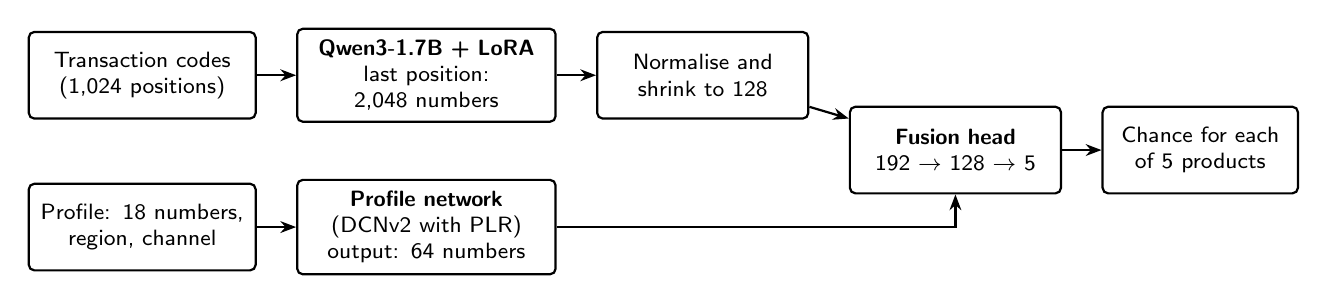
\begin{tikzpicture}[node distance=5mm and 5mm]
\node[box,text width=26mm] (ids) {Transaction codes\\(1,024 positions)};
\node[box,text width=30mm,right=of ids] (qwen) {\textbf{Qwen3-1.7B + LoRA}\\last position: 2,048 numbers};
\node[box,text width=24mm,right=of qwen] (proj) {Normalise and\\shrink to 128};
\node[box,text width=26mm,below=8mm of ids] (tab) {Profile: 18 numbers,\\region, channel};
\node[box,text width=30mm,right=of tab] (dcn) {\textbf{Profile network}\\(DCNv2 with PLR)\\output: 64 numbers};
\node[box,text width=24mm,right=of proj,yshift=-9.5mm] (mlp) {\textbf{Fusion head}\\192 $\rightarrow$ 128 $\rightarrow$ 5};
\node[box,text width=22mm,right=of mlp] (out) {Chance for each\\of 5 products};
\draw[arr] (ids) -- (qwen); \draw[arr] (qwen) -- (proj); \draw[arr] (proj) -- (mlp);
\draw[arr] (tab) -- (dcn); \draw[arr] (dcn) -| (mlp); \draw[arr] (mlp) -- (out);
\end{tikzpicture}
\caption{Our joint model. All trainable parts learn together from one loss on the offered product.}
\end{figure}

\begin{itemize}
\item \textbf{Profile network.} Each number is first expanded with sine and cosine features (PLR embeddings), which helps neural networks use numeric inputs. Three ``cross'' layers (DCNv2) then learn combinations of features, such as income together with region.
\item \textbf{Fusion head.} The transaction summary (128 numbers) and the profile summary (64 numbers) are joined and passed through a small network that outputs one score per product. During training, only the score of the product actually offered is compared with the outcome.
\item \textbf{Why train together.} Because one loss updates both branches, the language model is pushed to learn what the profile features miss.
\end{itemize}

\subsection{Fine-tuning setup}
\begin{tabularx}{\linewidth}{@{}L{4.3cm}X@{}}
\toprule
\textbf{Setting} & \textbf{Value and reason} \\
\midrule
Method & LoRA: small trainable add-on matrices inside the frozen model \\
LoRA rank / scale / dropout & 16 / 32 / 0.05 \\
LoRA placed on & All 7 projection layers (query, key, value, output, gate, up, down) in all 28 layers \\
Trainable parameters & 18.3 million in total, about 1\% of the model (17.4M LoRA + special-code table + heads) \\
Optimiser & AdamW; learning rate 2e-4 for LoRA, 1e-3 for the heads \\
Schedule & 5\% warm-up, then cosine decay; gradient clipping at 1.0 \\
Batch & 4 customers $\times$ 8 accumulation steps = 32 per update; 414 updates (1 pass) \\
Memory saving & 16-bit mixed precision with loss scaling; gradient checkpointing \\
Model selection & Validation AUC checked 4 times; best checkpoint kept \\
Peak GPU memory & 7.0\,GB of 16\,GB \\
Training time & 4.1 hours (transactions-only), 4.3 hours (joint), in parallel \\
\bottomrule
\end{tabularx}

%=====================================================================
\needspace{16\baselineskip}
\section{Code used for fine-tuning}
The full training script is a single Kaggle script of about 500 lines. The excerpts below are lightly trimmed for reading.

\begin{lstlisting}[caption={Building each customer's code sequence, newest transactions first until the window is full.}]
edges  = np.quantile(log_amount[train_rows], np.linspace(0, 1, 22)[1:-1])   # 21 amount ranges, train only
bucket = np.searchsorted(edges, log_amount, side="right")
head = np.stack([TX, sign, AMT_0 + bucket, MON_1 + month - 1, DAY_1 + day - 1, WD_0 + weekday], 1)

for start, end in customer_ranges:
    pieces, total = [], 0
    for i in range(end - 1, start - 1, -1):                 # walk back from the newest transaction
        p = list(head[i]) + desc_ids[descs[i]][:6]           # 6 codes + first 6 word-pieces
        if total + len(p) > 1024: break
        pieces.append(p); total += len(p)
    seqs[customer] = [t for p in reversed(pieces) for t in p]
\end{lstlisting}

\begin{lstlisting}[caption={Loading Qwen3-1.7B, adding LoRA, and the separate table for the 74 special codes.}]
lm = AutoModelForCausalLM.from_pretrained("Qwen/Qwen3-1.7B", torch_dtype=torch.float16)
backbone = lm.model                                          # drop the word-prediction layer
for p in backbone.parameters(): p.requires_grad_(False)     # freeze the base model
backbone = get_peft_model(backbone, LoraConfig(r=16, lora_alpha=32, lora_dropout=0.05,
           target_modules=["q_proj","k_proj","v_proj","o_proj","gate_proj","up_proj","down_proj"]))
backbone.gradient_checkpointing_enable()

special = nn.Embedding(74, 2048)                             # started from matching words' meanings
special.weight.data.copy_(init_from_words)

def encode(ids, mask):
    is_special = ids >= V0
    x = torch.where(is_special[..., None], special(ids - V0), word_embeddings(ids))
    h = backbone(inputs_embeds=x, attention_mask=mask).last_hidden_state
    return h[:, -1]                                          # left padding: last position is newest
\end{lstlisting}

\begin{lstlisting}[caption={The fusion head: one score per product; training uses the offered product's score.}]
class Head(nn.Module):
    def __init__(self, hidden, n_num, cat_sizes):
        super().__init__()
        self.ln   = nn.LayerNorm(hidden)
        self.proj = nn.Sequential(nn.Linear(hidden, 128), nn.ReLU())
        self.dcn  = DCNv2(n_num, cat_sizes)                  # profile network, 64 outputs
        self.mlp  = nn.Sequential(nn.Linear(192, 128), nn.ReLU(), nn.Dropout(0.1), nn.Linear(128, 5))
    def all_logits(self, h, xn, xc):
        z = torch.cat([self.proj(self.ln(h)), self.dcn(xn, xc[:, :2])], 1)
        return self.mlp(z)                                   # (batch, 5 products)
    def forward(self, h, xn, xc):
        return self.all_logits(h, xn, xc).gather(1, xc[:, 2:3]).squeeze(1)   # offered product
\end{lstlisting}

\begin{lstlisting}[caption={Training loop: mixed precision, gradient accumulation, clipping, and keeping the best checkpoint.}]
opt = torch.optim.AdamW([{"params": lora_params, "lr": 2e-4},
                         {"params": head.parameters(), "lr": 1e-3}])
scaler = torch.amp.GradScaler("cuda")
for batch, ids, mask, xn, xc, y in batches(train, size=4, shuffle=True):
    with torch.autocast("cuda", dtype=torch.float16):
        h = encode(ids, mask)
    loss = F.binary_cross_entropy_with_logits(head(h, xn, xc), y) / 8
    scaler.scale(loss).backward(); micro += 1
    if micro % 8: continue                                   # accumulate 8 batches
    set_lr(step); scaler.unscale_(opt)
    torch.nn.utils.clip_grad_norm_(trainable, 1.0)
    scaler.step(opt); scaler.update(); opt.zero_grad(); step += 1
    if step % eval_every == 0:
        val_auc = auc(y_val, score(val))
        if val_auc > best: best = val_auc; save_checkpoint()
\end{lstlisting}

\begin{lstlisting}[caption={Running the two fine-tuning jobs in parallel, one per GPU.}]
procs = [subprocess.Popen([python, script, "--worker", mode, "--gpu", str(g)])
         for g, mode in ((0, "seq"), (1, "joint"))]
return_codes = [p.wait() for p in procs]
report()                                                     # baselines, scores, charts
\end{lstlisting}

%=====================================================================
\section{Experiments and results}
\subsection{Models compared}
\begin{tabularx}{\linewidth}{@{}L{4.6cm}X@{}}
\toprule
\textbf{Model} & \textbf{What it uses} \\
\midrule
Standard model (LightGBM) & Profile features only; up to 3,000 trees with early stopping. \\
Two-step model & Transaction summary from the fine-tuned model, reduced to 32 numbers and added to LightGBM. \\
\textbf{Our model (joint)} & Transactions and profile, trained together end to end. \\
Profile details only & The profile network (DCNv2 with PLR) on its own. \\
Transactions only & The fine-tuned language model with a small head, no profile. \\
Highest possible & The true chances from the generator; the upper limit for any model. \\
\bottomrule
\end{tabularx}

\subsection{Scores}
AUC measures how often a model ranks a customer who took the product above one who did not: 0.5 is random guessing and 1.0 is perfect. All scores are on the same 5,069 test customers, of whom 12.9\% took the offered product.

\begin{figure}[!htb]
\centering
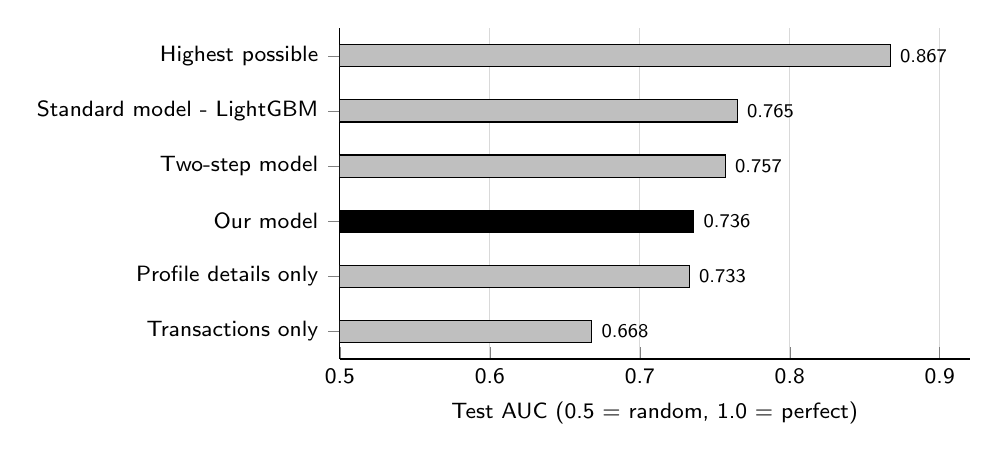
\begin{tikzpicture}
\begin{axis}[xbar, scale only axis, width=8cm, height=4.2cm, bar width=8pt, bar shift=0pt,
  xmin=0.5, xmax=0.92, xtick={0.5,0.6,0.7,0.8,0.9}, xticklabels={0.5,0.6,0.7,0.8,0.9},
  xlabel={Test AUC (0.5 = random, 1.0 = perfect)},
  symbolic y coords={Highest possible,Standard model - LightGBM,Two-step model,Our model,Profile details only,Transactions only},
  ytick={Highest possible,Standard model - LightGBM,Two-step model,Our model,Profile details only,Transactions only},
  y dir=reverse, enlarge y limits=0.1, point meta=explicit symbolic, nodes near coords,
  nodes near coords style={font=\scriptsize,anchor=west}, every axis label/.style={font=\footnotesize},
  tick label style={font=\footnotesize}, axis x line*=bottom, axis y line*=left, xmajorgrids, grid style={black!15}]
\addplot[draw=black, fill=black!25] coordinates {(0.867,Highest possible)[0.867] (0.765,Standard model - LightGBM)[0.765] (0.757,Two-step model)[0.757] (0.733,Profile details only)[0.733] (0.668,Transactions only)[0.668]};
\addplot[draw=black, fill=black] coordinates {(0.736,Our model)[0.736]};
\end{axis}
\end{tikzpicture}
\caption{Test AUC of every model after round 2. Our model is the black bar.}
\end{figure}

\begin{table}[!htb]
\centering\footnotesize
\begin{tabular}{@{}lrrrrr@{}}
\toprule
\textbf{Model} & \textbf{AUC} & \textbf{vs standard} & \textbf{PR-AUC} & \textbf{Top product right} & \textbf{Rank agreement} \\
\midrule
Standard model (LightGBM) & 0.765 & -- & 0.372 & 56\% & 0.63 \\
Two-step model & 0.757 & $-$1.0\% & 0.379 & 54\% & 0.59 \\
\textbf{Our model (joint)} & \textbf{0.736} & \textbf{$-$3.8\%} & \textbf{0.332} & \textbf{44\%} & \textbf{0.49} \\
Profile details only & 0.733 & $-$4.2\% & -- & 45\% & 0.52 \\
Transactions only & 0.668 & $-$12.7\% & 0.240 & 32\% & 0.22 \\
Highest possible & 0.867 & +13.3\% & -- & 100\% & 1.00 \\
\bottomrule
\end{tabular}
\caption{All results. PR-AUC focuses on the customers who took the product (12.9\% would be random). ``Top product right'' is how often the model's top product matches the true best product (20\% would be random). ``Rank agreement'' compares each model's order of the five products with the true order (0 = no agreement, 1 = identical).}
\end{table}

\subsection{Round 1 compared with round 2}
Round 1 read the last 512 codes (about 37 transactions) and treated the offered product as an input. Round 2 doubled the window to 1,024 codes (about 87 transactions), capped merchant names at 6 word-pieces, and gave each product its own output.

\begin{figure}[!htb]
\centering
\begin{minipage}[t]{0.47\linewidth}\centering
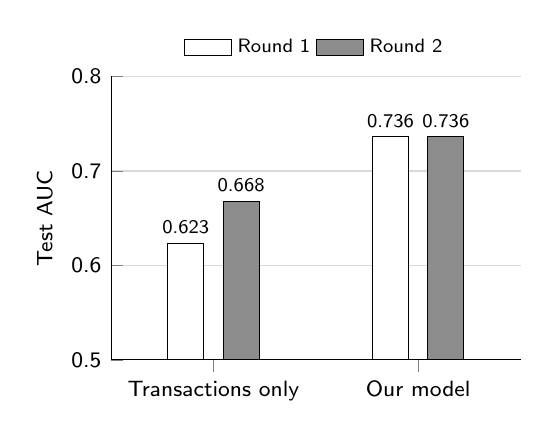
\begin{tikzpicture}
\begin{axis}[ybar=7pt, scale only axis, width=5.2cm, height=3.6cm, bar width=13pt,
  ymin=0.5, ymax=0.8, ytick={0.5,0.6,0.7,0.8}, yticklabels={0.5,0.6,0.7,0.8}, ylabel={Test AUC},
  symbolic x coords={Transactions only,Our model}, xtick=data, enlarge x limits=0.5,
  point meta=explicit symbolic, nodes near coords, nodes near coords style={font=\scriptsize},
  area legend, legend style={font=\scriptsize,at={(0.5,1.03)},anchor=south,legend columns=2,draw=none},
  every axis label/.style={font=\footnotesize}, tick label style={font=\footnotesize},
  axis x line*=bottom, axis y line*=left, ymajorgrids, grid style={black!15}]
\addplot[draw=black, fill=white] coordinates {(Transactions only,0.623)[0.623] (Our model,0.736)[0.736]};
\addplot[draw=black, fill=black!45] coordinates {(Transactions only,0.668)[0.668] (Our model,0.736)[0.736]};
\legend{Round 1, Round 2}
\end{axis}
\end{tikzpicture}
\caption{Test AUC in each round.}
\end{minipage}\hfill
\begin{minipage}[t]{0.47\linewidth}\centering
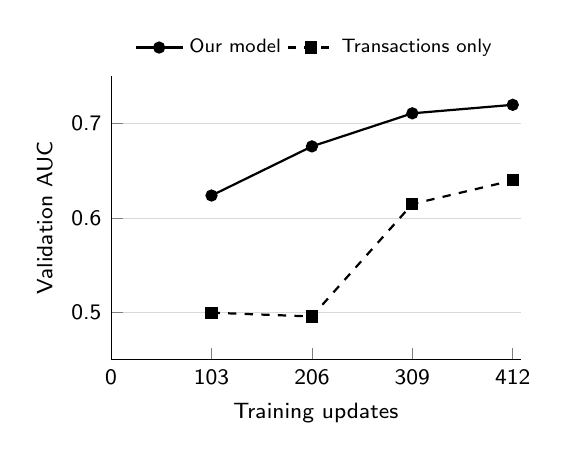
\begin{tikzpicture}
\begin{axis}[scale only axis, width=5.2cm, height=3.6cm, xmin=0, xmax=420, ymin=0.45, ymax=0.75,
  xtick={0,103,206,309,412}, xticklabels={0,103,206,309,412}, ytick={0.5,0.6,0.7}, yticklabels={0.5,0.6,0.7},
  xlabel={Training updates}, ylabel={Validation AUC},
  legend style={font=\scriptsize,at={(0.5,1.03)},anchor=south,legend columns=2,draw=none},
  every axis label/.style={font=\footnotesize}, tick label style={font=\footnotesize},
  axis x line*=bottom, axis y line*=left, ymajorgrids, grid style={black!15}]
\addplot[thick, black, mark=*, mark size=1.8pt] coordinates {(103,0.624) (206,0.676) (309,0.711) (412,0.720)};
\addplot[thick, black, dashed, mark=square*, mark size=1.8pt, mark options={solid}] coordinates {(103,0.500) (206,0.496) (309,0.615) (412,0.640)};
\legend{Our model, Transactions only}
\end{axis}
\end{tikzpicture}
\caption{Validation AUC during round 2 training.}
\end{minipage}
\end{figure}

\begin{table}[!htb]
\centering\footnotesize
\begin{tabular}{@{}lrrl@{}}
\toprule
\textbf{Model} & \textbf{Round 1} & \textbf{Round 2} & \textbf{Change (95\% range from resampling the test set)} \\
\midrule
Transactions only & 0.623 & 0.668 & +0.045 (+0.029 to +0.062): a real improvement \\
Our model (joint) & 0.736 & 0.736 & +0.0005 ($-$0.009 to +0.010): no change \\
\bottomrule
\end{tabular}
\caption{Round 1 vs round 2 on the same test customers, with a paired bootstrap of 2,000 resamples.}
\end{table}

\subsection{What the results show}
\begin{itemize}
\item \textbf{Transaction history carries real signal.} On its own it reaches 0.668, and reading more history improved it clearly.
\item \textbf{Our model does not yet beat the standard model.} It is 3.8\% below LightGBM. Its edge over the profile network alone (0.736 vs 0.733) is too small to separate from test noise.
\item \textbf{Validation scores were still rising} at the end of the single training pass (0.711 to 0.720), which suggests more training would help.
\item \textbf{The test set limits what we can measure.} With 5,069 customers, AUC is accurate to about $\pm$0.022. Gains smaller than that need a larger test set.
\end{itemize}

%=====================================================================
\section{Problems found and how we solved them}
\begin{tabularx}{\linewidth}{@{}L{3.6cm}XL{3.2cm}@{}}
\toprule
\textbf{Problem} & \textbf{What we did} & \textbf{Result} \\
\midrule
No real bank data & Built a generator that also stores each customer's true chance per product & Highest possible score is known \\
Transactions as text are long; amounts read poorly & Six compact codes per transaction plus a short merchant name & 11.7 codes per transaction \\
Enlarging the vocabulary would add 311M parameters & Separate 74-entry table for the special codes & Base vocabulary unchanged \\
Model too large to fully train on free GPUs & LoRA (about 1\% trainable), 16-bit maths, gradient checkpointing & 7\,GB peak memory \\
Risk of testing on seen data & Split by month; amount ranges and scaling fitted on training data only & Fair test on future customers \\
Library conflict on Kaggle (PEFT and torchao) & Disabled the unused torchao check at start-up & Training runs cleanly \\
Round 1 saw only 37 transactions & Doubled the window; capped merchant names at 6 word-pieces & Transactions-only AUC 0.623 $\rightarrow$ 0.668 \\
Round 1 ranked products worse than chance & One output per product instead of the offer as an input & Rank agreement $-$0.22 $\rightarrow$ +0.22 \\
\bottomrule
\end{tabularx}

%=====================================================================
\section{Limitations}
\begin{itemize}
\item \textbf{Small training set.} 13,265 training customers and one pass of 414 updates.
\item \textbf{No spending-pattern pre-training.} Qwen3 learned from general web text; it has never been taught how bank transactions usually follow each other.
\item \textbf{Synthetic data.} The generator encodes our assumptions about behaviour. Real data will differ, and in this generator the 90-day totals already capture much of the signal.
\item \textbf{One outcome per customer.} We only see whether the customer took the product they were offered, not the other four.
\item \textbf{Two changes in round 2 at once.} The window size and the output head changed together, so their separate effects are unknown.
\end{itemize}

%=====================================================================
\section{Suggested steps to improve the results}
\begin{enumerate}
\item \textbf{Teach the model spending patterns first.} Train it to predict the next transaction across all 4.25 million transactions (no labels needed), then fine-tune it for recommendation. This is expected to give the largest gain.
\item \textbf{Use more customers and train longer.} Generate 50,000 or more training customers and train for three passes instead of one; validation scores were still rising.
\item \textbf{Use a larger test set.} About 55,000 test customers are needed to measure a 1\% improvement reliably.
\item \textbf{Change one thing at a time.} Run separate rounds for window size, head design and learning rate, so each effect is known.
\item \textbf{Get more computing time.} Round 2 used 6.4 of Kaggle's 12 free hours. Longer training needs a paid GPU or a multi-session setup that resumes from checkpoints.
\item \textbf{Try a longer window and a stronger profile model.} A 2,048-code window would cover about 4 months; adding LightGBM's predictions as an input to the fusion head may also help.
\item \textbf{Test on real, anonymised bank data} to confirm the results hold outside the synthetic setting.
\end{enumerate}

%=====================================================================
\section*{Appendix: how to reproduce}
\begin{enumerate}
\item Generate the data: \texttt{python -m synthgen.generate -{}-n-users 20000 -{}-seed 7 -{}-out data/}
\item Upload \texttt{data/} as a Kaggle dataset and attach the Qwen3-1.7B model.
\item Run the training script as a Kaggle notebook with 2$\times$T4 GPUs. It prepares the data, runs both fine-tuning jobs in parallel, trains the baselines and writes \texttt{results.json} and the charts.
\item For a quick local test without a GPU: run the training script with \texttt{-{}-smoke}.
\end{enumerate}
Total run time for round 2: 386 minutes. All random seeds are fixed (generator 7, training 42).

\end{document}
